\documentclass[12pt, a4paper]{article}
% pacotes utilizados
%\usepackage{abnt-UFPR}
\usepackage[pdftex]{graphicx}
\usepackage{graphicx,url}
\usepackage[utf8]{inputenc}
\usepackage[brazil]{babel}
\usepackage{setspace}
\onehalfspace
\usepackage{enumerate}
\usepackage{multirow}
\usepackage{parskip}
\usepackage{float}
\usepackage{color}
\usepackage[normalem]{ulem}
\usepackage{lmodern}
\usepackage{pdfpages}

\usepackage{listings}

\definecolor{verdao}{rgb}{0.0, 0.5, 0.0}

\lstset{
	language=Python,
	frame=single,
	numbers=left,
	showspaces=false,
	showstringspaces=false,
	basicstyle=\ttfamily,
	captionpos=t,
	basicstyle=\small,
	keywordstyle=\ttfamily \color{blue},
	keywordstyle=[2]\ttfamily \color{blue},
	stringstyle=\color{red}\ttfamily,
	commentstyle=\color{verdao}\ttfamily
}

%\usepackage{fancyhdr}
\usepackage{indentfirst}
\usepackage[a4paper,left=3cm,right=2cm,top=3cm,bottom=2cm]{geometry}
\usepackage[alf]{abntex2cite}
%\pagestyle{headings}
%configuracoes do sumario
\usepackage{tocloft}
\renewcommand{\cftdot}{\textbf{.}}
\renewcommand{\cftsecdotsep}{\cftdotsep}
\renewcommand{\cftsecdotsep}{4}
\renewcommand{\cftsubsecdotsep}{4}
\renewcommand{\cftsecfont}{\normalsize\bfseries}
\renewcommand{\cftsubsecfont}{\normalsize}
\renewcommand{\cftsecpagefont}{\textbf}
\renewcommand{\cftsubsecpagefont}{\textbf}
\cftsetindents{section}{0cm}{1.3cm}
\cftsetindents{subsection}{0cm}{1.3cm}
\cftsetindents{subsubsection}{0cm}{1.3cm}
%\renewcommand{\figurename}{Fig.}
\newcommand{\bigsize}{\fontsize{12pt}{20pt}\selectfont}

\usepackage[labelsep=endash]{caption}
\setlength{\cftsubsecindent}{0em}
\tocloftpagestyle{empty}
\newcommand{\bfemph}[1]{\textbf{\textit{#1}}}
\renewcommand{\emph}[1]{\bfemph{#1}}
%Formatacao de Padroes das Referencias Bibliograficas
%\usepackage{custom-bib}

%Formatacao de Titulos, Secoes, Subtitulos, etc...
\usepackage{titlesec}
\titleformat{\section}{\normalfont\normalsize\filright\bfseries}{\thesection}{1em}{\uppercase}
%\renewcommand{\thesubsection}{\alph{subsection}}
\titleformat{\subsection}{\normalfont\normalsize\filright\bfseries}{\thesubsection}{1em}{}
%\renewcommand{\thesubsubsection}{\roman{subsubsection}}
\titleformat{\subsubsection}{\normalfont\normalsize\bfseries}{\thesubsubsection}{1em}{}
%

%Espacamento de Paragrafos
\setlength{\parindent}{0.8cm}
\setlength{\parskip}{1ex plus 0.5ex minus 0.2ex}
%1ex plus 0.5ex minus 0.2ex
\pagestyle{myheadings}

\pagenumbering{arabic}

\author{ \bf UNIVERSIDADE DO ESTADO DO AMAZONAS - UEA \\[14pt] \small ESCOLA SUPERIOR DE TECNOLOGIA - EST \\[14pt] ENGENHARIA ELÉTRICA \\[96pt] CARLA PATRICIA MICHILES ARAUJO \\[96pt]}
\title{ \rm \bf \Large SISTEMA DE AQUISIÇÃO DE SINAIS ELETROCARDIOGRÁFICOS UTILIZANDO TECNOLOGIA WIRELESS\\[123pt] \rm \small Manaus \\  2018}




\pagestyle{myheadings}

% Start the document
\begin{document}

\addtocontents{toc}{\protect\thispagestyle{empty}}
%INÍCIO DA CAPA DA MONOGRAFIA
\thispagestyle{empty}
\begin{center}
\textbf{ UNIVERSIDADE PAULISTA \\
CIÊNCIAS DA COMPUTAÇÃO \\[50pt] }
\textbf{ \\[70pt] {\bigsize GIOVANNI JUNIOR ROSSINI} \\
GUILHERME HENRIQUE VARGAS\\[120pt] }
\textbf{ {\bigsize ANÁLISE DE SENTIMENTOS PARA RECONHECER AGRESSÕES RACIAIS NAS REDES E MÍDIAS SOCIAIS}  \\[104pt] }
\end{center}
% COMENTÁRIOS DA FOLHA DE ROSTO
\hspace*{8cm}

\vspace*{\fill}

\begin{center}
Bauru \\ 2018
\end{center}

%FIM DA CAPA DA MONOGRAFIA

%INÍCIO DA FOLHA DE ROSTO
\newpage
\thispagestyle{empty}
\begin{center}


% \textbf{ \\[70pt] {\bigsize CARLA PATRICIA MICHILES ARAUJO} \\[120pt] }
\textbf{ {\bigsize GIOVANNI JUNIOR ROSSINI} \\
GUILHERME HENRIQUE VARGAS \\[120pt] }
\textbf{ {\bigsize  ANÁLISE DE SENTIMENTOS PARA RECONHECER AGRESSÕES RACIAIS NAS REDES E MÍDIAS SOCIAIS}  \\[50pt] }
\end{center}
% COMENTÁRIOS DA FOLHA DE ROSTO
\hspace*{8cm}
\begin{flushright}
\begin{minipage}{8cm}
\begin{singlespace}
Projeto de pesquisa desenvolvido durante a disciplina de Trabalho de Conclusão de Curso e apresentada à banca avaliadora do Curso de Ciências da Computação da Universidade Paulista, como pré-requisito para obtenção do título de Cientista da Computação.\\[50pt]
\end{singlespace}
\end{minipage}
\end{flushright}
\begin{center}
Orientador: Robson Fernandes

\end{center}

\vspace*{\fill}
\begin{center}
Bauru \\ 2018
\end{center}

%FIM DA FOLHA DE ROSTO

\newpage

\thispagestyle{empty}
\vspace*{4.4cm}
{\begin{center}\textbf{\normalsize RESUMO}\vspace{36pt}\end{center}}
Com a scensão das mídias sociais, como blogs e redes sociais, têm despertado o interesse em análise de sentimentos. Com a proliferação de opiniões, avaliações, recomendações e outras formas de expressões on-line, a opinião se transformou em uma importante ferramenta tanto para pesquisas, empresas, fornecedores, entre outros. Essa tarefa de identificar se a opinião que foi expressada em um determinado texto, é positiva ou negativa permite tomar ações específicas, assim como denunciar abusos e discriminações. Dessa forma garantir como prova racional e lógica que textos como \textit{tweets, post} no Facebook e textos de mídias sociais como blog, revistas digitais entre outros meios podem e contém textos racistas e discriminatórios.
Utilizando métodos de análise de dados para analisar um texto, quantificar o número de palavras, as vezes nas quais elas se repetem e em quais situações são repetidas, esse texto passa por um processo de pontuação, onde cada palavra tem uma pontuação tornando ela positiva ou negativa. Ao final teremos uma estátistica precisa de como as mídias sociais geram grandes números de discriminações raciais.


\textbf{Palavras chave}: análise de sentimentos, mineração de dados, mídias sociais, redes sociais, lexicon, discriminação racial
\newpage
\thispagestyle{empty}
\vspace*{4.4cm}
{\begin{center}\textbf{\normalsize ABSTRACT}\vspace{36pt}\end{center}}
With the spread of social media, such as blogs and social networks, have aroused interest in sentiment analysis. With the proliferation of opinions, evaluations, recommendations and other forms of on-line expression, opinion has become an important tool for research, companies, suppliers, and others. This task of identifying whether the opinion expressed in a given text is positive or negative allows specific actions to be taken, as well as denouncing abuses and discrimination. In this way, to guarantee as rational and logical proof that texts such as tweets, post on Facebook and social media texts such as blog, digital magazines among other means can and do contain racist and discriminatory texts. Using data analysis methods to analyze a text, quantify the number of words, the times in which they are repeated and in which situations are repeated, this text goes through a punctuation process, where each word has a punctuation making it positive or negative. At the end we will have a precise statistics on how social media generate large numbers of racial discrimination.


\textbf{Keywords}: Sentiment analysis, data mining, social media, social networks, lexicon, racial discrimination.


%INÍCIO DA LISTA DE FIGURAS

\newpage
\pagestyle{empty}
\vspace*{4cm}
\listoffigures
\clearpage
%\pagestyle{plain}
%FIM DA LISTA DE FIGURAS



%INÍCIO DO SUMÁRIO
\newpage
\pagestyle{empty}
\vspace*{3.5cm}
\renewcommand{\contentsname}{\begin{center}\textbf{\normalsize SUMÁRIO}\vspace{36pt}\end{center}}
\tableofcontents
\clearpage
%FIM DO SUMÁRIO
\pagestyle{myheadings}

%INÍCIO DO CAPÍTULO 1 - INTRODUÇÃO
\newpage
\vspace*{4cm}

%\fancypagestyle{plain}{
%  \fancyhf{}% Clear header/footer
%  \fancyhead[R]{}% Right header
%  \fancyfoot[L]{}% Left footer
%  \fancyfoot[R]{\thepage}% Right footer
%}

%\thispagestyle{fancy}

%\pagestyle{fancy}
%\renewcommand{\headrulewidth}{0pt}
%\rhead{\thepage}
%\fancyfoot[C]{}

%\fancyfoot[R]{\thepage}
\setcounter{page}{7}
\begin{center}
\textbf{INTRODUÇÃO\\}
\end{center}
\par
\addcontentsline{toc}{section}{INTRODUÇ\~AO}	

Deep Learning é o termo usado basicamente para apresentar o escopo de como se utilizar estruturas de redes neurais de múltiplas camadas e que podem ser aplicadas para uma incrível variedade de diferentes combinações de técnicas matemáticas. Esses modelos são incrivelmente poderosos, entretanto nossa habilidade de utilizar redes neurais de uma forma eficiente tem sido um fato relativamente novo, pois agora temos grandes quantidades de dados disponíveis (Big Data) e uma capacidade computacional que nos permite transformar os modelos de Deep Learning em uma técnica extremamente poderosa \cite{matos}.
Segundo Matos \citeyear{matos2} o diferencialdo Deep Learning está no fato que o modelo criado tem mais flexibilidade em determinar de qual maneira os dados serão utilizados para construir um resultado viável. O Cientista de Dados não tem que perder tanto tempo analisando para descobrir quais inputs devem ser incluídos, pois os modelos de Deep Learning podem considerar todos os parâmetros e de uma maneira perspicaz e determinar qual a melhor combinação dos valores de entrada. Isso torna o processo de tomada de decisão muito mais sofisticado, transformando computadores e dispositivos em sistemas com mais inteligência adaptativa do que nunca. Com Deep Learning podemos criar automóveis que por si próprios conseguem traçar uma rota com um destino final ou, telefones que compreendem nossa voz, sistemas para tradução de idiomas, reconhecimento facial, análise preditiva, composição de músicas por algoritmos e uma vasta plataforma onde outras aplicações de Inteligência Artificial estão se tornando viáveis graças ao Deep Learning.
Análise de sentimento é a ação que por si só tem a finalidade de identificar se a opinião que foi expressada em um determinado trecho, é realmente positiva ou negativa.
Para começar, é importante compreender que opiniões e sentimentos, bem como seus conceitos relacionados como avaliação, atitude, emoção e humor são influenciadores do respectivo comportamento humano. Nossas crenças e percepções sobre a realidade, assim como nossas escolhas, são bastante condicionadas com a forma que outras pessoas veem e percebem o mundo. Nossa visão do mundo, é muitas vezes influenciada pela visão e opinião de outras pessoas \cite{matos}

\newpage
\section{OBJETIVO}
%\pagestyle{fancy}
%\fancyhead{}
%\renewcommand{\headrulewidth}{0pt}
%\rhead{\thepage}
%\fancyfoot[C]{}

\subsection{OBJETIVO GERAL}
\hspace*{0.8cm}O objetivo deste trabalho é desenvolver uma aplicação utilizando Deep Learning para que, através da ação Análise de Sentimentos mostre e detecte textos racistas expostos por internautas em redes sociais.

\begin{figure}[H]
\centering
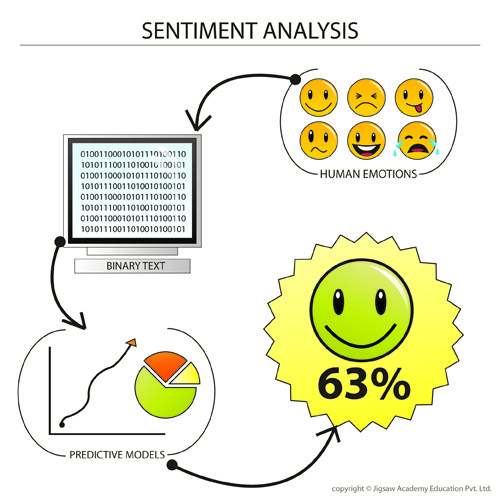
\includegraphics[width=.55\textwidth]{como_funciona.jpg}
\caption{Como funciona a análise de sentimentos}
\label{fig:Fig1}
\end{figure}
%Fonte: Jigsaw Academy Education.

\subsection{OBJETIVOS ESPECÍFICOS}
\begin{itemize}
\item Direcionar o foco da aplicação para detectar o racismo.
\item Coletar dados textuais com supostos racismos explícitos.
\item Aplicar Machine Learning para fazer com que, nossa aplicação tenha dados alimentados o suficiente para entender e determinar tal proposição.
\item Colocar a aplicação para trabalhar em diferentes tipos de situação.
\item Detectar palavras chaves.
\end{itemize}

\subsection{PROBLEMA}

\hspace*{0.8cm}Uma situação que desde sempre convivemos em nosso redor é o racismo, sendo alvo ou, presenciando eventos que envolvem terceiros. Com o crescimento da internet e redes sociais cresce também o número de ataques racistas que ocorrem a alguns internautas por meio de tal mídia. Visando este meio, o projeto aqui presente reúne recursos para detectar e denunciar textos racistas juntamente com o usuário que a expõe. 

\subsection{JUSTIFICATIVA}

\hspace*{0.8cm}A jornalista Maria Júlia Coutinho, conhecida comoMaju, que apresenta a previsão do tempo no Jornal Nacional, da Rede Globo, foi alvo decomentários racistasno Facebook. Uma publicaçãodo JN do final da quinta-feira na rede social, sobre o tempo na região central do Brasil, foi comentada mais de 7 mil vezes, muitas com injúrias raciais à jornalista.

O zagueiro Rafael Vaz sentiu tristeza, raiva, vontade de brigar e de chorar – tudo junto – quando viu que sua foto no Instagram, ao lado de sua filha Raphaella, recebeu comentários com a palavra “macaco” e outras que não podem ser publicadas. Sete meses depois do episódio, ficou o receio, quase medo, de usar as redes sociais novamente. “Fico com receio de que aconteça de novo. Penso três vezes antes de postar qualquer coisa. Na internet, as pessoas sabem que não serão pegas. Quem fez uma vez, vai fazer de novo”, diz o defensor do Flamengo. 
Abaixo temos uma estatística de como vem sido o progresso de discriminações raciais ao passar dos anos:

\begin{figure}[H]
\centering
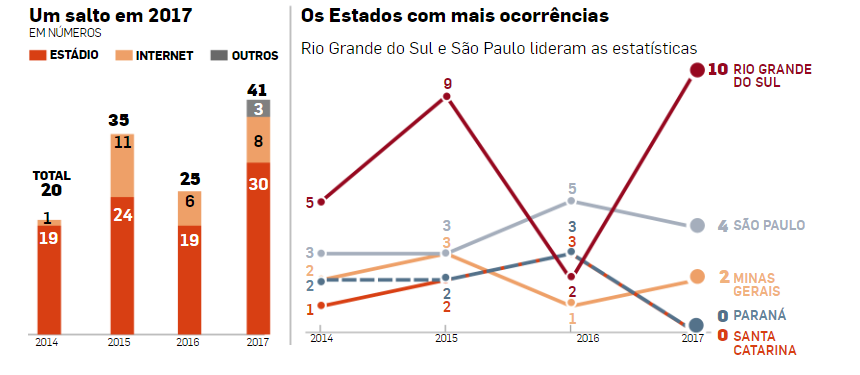
\includegraphics[width=.75\textwidth]{estatistica_estadao.png}
\caption{Casos registrados de discriminação}
\label{fig:Fig2}
\end{figure}
%Fonte: Observatório da Discriminação Racial do Futebol Brasileiro, 2017.

\hspace*{0.8cm}Perante essas situações algumas vítimas acabam optando por não denunciar ou expor o agressor mesmo sabendo que é crime, pois os mesmos veem as estáticas referente ao problema crescendo ano após ano e a situação se repetindo, acabam decidindo assim, por si só absorver e aceitar o ataque.
As mesmas pessoas que praticam este ato por sua vez saem impunes, pois como o zagueiro Rafael Vaz citou, “Na internet, as pessoas sabem que não serão pegas”, casos como estes tende serem analisado e julgados, casos de racismo não deve ser crescente conforme nossa mídia cresce.

\newpage
\section{REFERENCIAL TEÓRICO}	

%\pagestyle{fancy}
%\fancyhead{}
%\renewcommand{\headrulewidth}{0pt}
%\rhead{\thepage}
%\fancyfoot[C]{}

\hspace*{0.8cm}Vários termos e conceitos vêm sendo descritos para tarefas associadas a detecção de sentimentos, diante da ascensão deste tema. A seguir é apresentada cada uma delas: 

Polaridade: Representa o grau de positividade e negatividade de um texto. Alguns métodos tratam a polaridade como um resultado discreto binário (positivo ou negativo) ou ternário (positivo, negativo ou neutro). Por exemplo, a frase “Como você está bonita hoje” é positiva e a frase “Hoje é um péssimo dia” é negativa, já a frase “Hoje é 21 de Outubro” não possui polaridade e normalmente é classificada como neutra.

Força do sentimento: É a representação da intensidade de um sentimento ou da polaridade, também é uma forma de saída de alguns métodos. Usualmente é um ponto flutuante entre -1 e 1 que torna, muitas vezes, necessário o uso de um limiar estabelecido de acordo com as características dos objetos que se quer isolar para identificar a neutralidade de uma sentença.

Sentimento/Emoção: Indica um sentimento específico presente em uma mensagem (ex.: raiva, surpresa, felicidade, etc.). Alguns métodos são capazes de identificar quais sentimentos em específico uma sentença representa. Como exemplo o método léxico Emolex \cite{Mohammad}, na qual é baseada a partir da avaliação de sentenças para 9 sentimentos diferentes: alegria, tristeza, raiva, medo, confiança, repugnância, surpresa, antecipação, positivo, negativo.

Subjetividade vs. Objetividade: Uma sentença objetiva possui normalmente um fato ou uma informação, enquanto sentenças subjetivas expressam sentimentos pessoais e opiniões. Algumas técnicas utilizam a análise da objetividade para estimar se compensa realizar a análise de sentimentos. Portanto entender se um conjunto de dados possui mais sentenças objetivas ou subjetivas pode influenciar diretamente os resultados. Cabe ressaltar que textos informais (ex.: coletados de redes sociais) tendem a ser mais subjetivos que textos formais (ex.: coletados de notícias).

\newpage
\subsection{OPINIÃO PUBLICA E MIDIAS SOCIAIS}
\hspace*{0.8cm}Com o avanço tecnológico a dissipação e a evolução dos portais especializados, blogs e redes sociais se tornam grandes meios de comunicação na Web 2.0 e com isso uma grande  5 quantidade opiniões, desde classificações e recomendações a resenhas e artigos, estão acessíveis e são acessados diariamente por uma grande parte da população mundial. Em uma visão sociológica, a opinião pública pode ser entendida como dinâmica, reativa e coletiva. Nos quais os públicos são moldados por técnicas que os representam, incluindo pesquisas, textos e outras formas de expressão pública \cite{Perrin}. Dessa forma, atualmente, torna-se lento e longo o processo de pesquisa das opiniões que podem ser obtidas na internet. Entretanto esse processo se tornou objeto de uma disciplina chamada “análise de sentimento”. Nesta disciplina o estudo de opiniões, identificação e extração de sentimentos e emoções expressas em textos na web é essencial para definirmos este conceito de “análise de sentimentos”.

\subsection{ONTOLOGIA}

\hspace*{0.8cm}Ontologia vem do grego e consiste em uma filosofia que estuda o que é inerente ao ser, sua existência e a realidade. “Qualquer estudo da opinião pública deve considerar o status ontológico do público que está sendo representado” \cite{Perrin}. Segundo Cicortas, Iordan e Fortis \citeyear{Cicortas}, sistemas de informação projetados para interpretar a linguagem humana estão em ascensão e que, com a mínima intervenção humana, serão capazes de entender as emoções, intenções e opiniões de um autor. Os autores em seu artigo chamado \textit{Considerations on Construction Ontologies}, caracterizam as dificuldades que ferramentas automatizadas têm em interpretar as informações e analisam as possibilidades do uso da ontologia para resolver tais questões. Em busca de melhores práticas para a construções ontológicas, os autores Rosner e Kunze \citeyear{Kunze} expõem suas experiências e perguntas sobre tais construções e detalham vários métodos para o aproveitamento das restrições da linguagem.

\newpage
\subsection{MÉTODOS DE ANÁLISE DE SENTIMENTOS}

\hspace*{0.8cm}Existem inúmeros modos de realizar análise de sentimentos. Devido as técnicas de previsão de sentimentos, esses métodos se diferem com o uso do aprendizado de máquinas, dicionários, processamento e escalas. Nosso trabalho focará nos métodos que buscam a detecção em pequenas subdivisões, assumindo que cada frase é capaz de possuir um único  6 sentimento central \cite{Liu}. Em seguida, apresentaremos os métodos de análise de sentimentos que pretendemos utilizar neste trabalho e que serão abordados na seção de Métodos e Materiais.

LIWIC que é uma ferramenta para análise de texto que, segundo Tausczik e Pennebaker \citeyear{Tausczik}, consegue estimar componentes psicológicos, estruturais e emocionais de um texto no uso de um dicionário onde as palavras estão categorizadas, podendo assim detectar a pontuação de polaridade positiva ou negativa.

SentiStrength consegue estimar a força do sentimento positivo e negativo em textos curtos, até em linguagem informal. Tem precisão de nível humano classificando de -5 (extremamente negativo) a 5 (extremamente positivo).

SentiWordNet é um recurso léxico para a mineração de opinião. Ele atribui a cada sincronia três pontuações de sentimento: positivo, negativo e neutro.

SASA é uma ferramenta de análise de sentimentos com modelos treinados em dados do Twitter.

Happiness Index, segundo Dodds and Danforth \citeyear{Dodds}, é uma escala de sentimentos que utiliza o Affective Norms for English Words (ANEW). O ANEW é uma coleção de 1.034 palavras associadas as dimensões afetivas de sentimentos. O Happiness Index foi gerado com base no ANEW e pontua um texto com valores entre 1 e 9, que indica o quão “feliz” o texto é. Após os cálculos efetuados em base da quantidade de vezes que cada palavra aparece no ANEW ele tira a média onde o intervalo entre 1 e 5 como negativos e 5 e 9 como positivos.

PANAS-t é uma escala psicométrica para a medição de sentimentos que permite detectar sentimentos do público sobre eventos utilizando uma base de dados extraída do Twitter \cite{Goncalves}.

NRC Hashtag Sentiment Lexicon utiliza do NRC Emotion Lexicon que é uma coleção de sete léxicos, incluindo o Word-Emotion Association Lexicon. Cada léxico tem uma lista de palavras e suas associações com certas categorias de interesse, como emoções (alegria, tristeza, medo, etc.), sentimento (positivo e negativo) ou cor (vermelho, azul, preto, etc.) \cite{nrcc}, para utilização e analise de hashtags no Twitter.

WAL é uma extensão do WordNet Domains, que inclui um subconjunto de conjunto de sinônimos adequados para representar conceitos afetivos correlacionados com palavras afetivas. Onde é atribuído um número de sintetizadores do WordNet um ou mais rótulos afetivos.

VADER é uma ferramenta de análise de sentimentos baseada em léxicos e regras que é especificamente sintonizada com sentimentos expressos em mídias sociais.

Abaixo, de uma forma generalizada de como funciona um método de análise de sentimentos:

\begin{figure}[H]
\centering
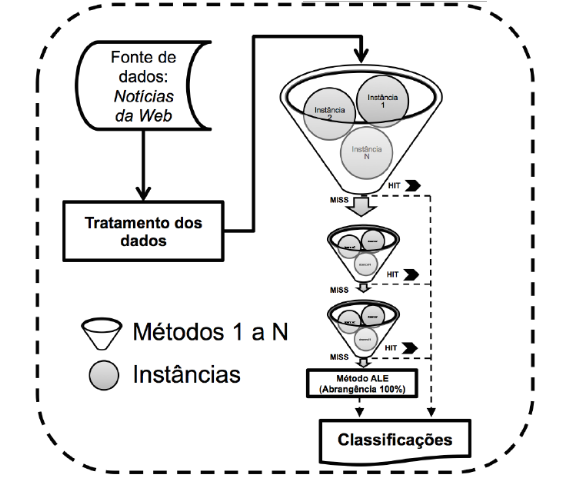
\includegraphics[width=.50\textwidth]{tecnica_de_analise.png}
\caption{Representação gráfica que métodos de Analise de Sentimentos utilizam}
\label{fig:Fig3}
\end{figure}
%Fonte: ResearchGate.

\newpage
\section{Materiais e Métodos}
%\pagestyle{fancy}
%\fancyhead{}
%\renewcommand{\headrulewidth}{0pt}
%\rhead{\thepage}
%\fancyfoot[C]{}

A pesquisa desenvolvida neste trabalho consiste de duas etapas, a primeira trata-se de uma pesquisa bibliográfica a qual visa reunir as informações e dados que servirão de base para a construção da investigação proposta.

O levantamento bibliográfico será feito a partir da análise de fontes as quais podem ser livros, artigos, documentos monográficos, periódicos (jornais, revistas, etc), textos disponíveis em sites confiáveis, entre outros locais que apresentam um conteúdo documentado.

Após a seleção do material, o mesmo será lido, analisado e interpretado, para o correto entendimento de todo o assunto envolvido no tema deste trabalho.

A segunda etapa trata-se da parte prática da proposta deste trabalho a qual trata-se do desenvolvimento de um sistema de análise de sentimentos capaz de reconhecer textos agressivos perante a ideologias raciais.

Para esta segunda etapa os seguintes materiais são usados:

Softwares:

Python para a programação da inteligência artificial e ou deep learning.

\begin{figure}[H]
\centering
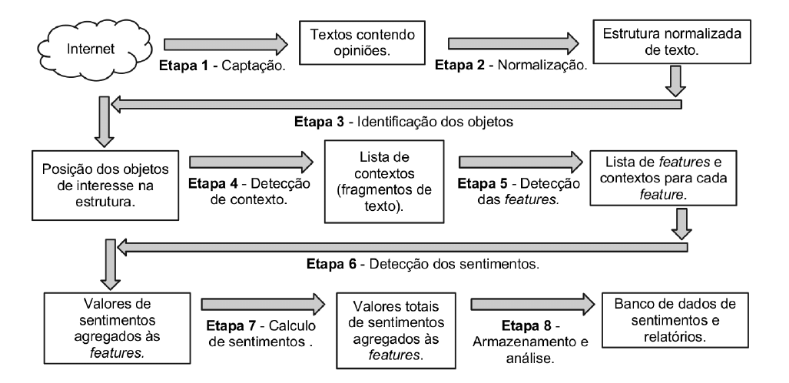
\includegraphics[width=.8\textwidth]{fluxograma.png}
\caption{Fluxograma de desenvolvimento}
\label{fig:Fig4}
\end{figure}
%Fonte: ResearchGate.

Hardware:

O hardware necessário neste trabalho consiste de:

Computador notebook com 12GB de memória e processador Intel i7-7th.

\subsection{Cronograma}
\begin{figure}[H]
\centering
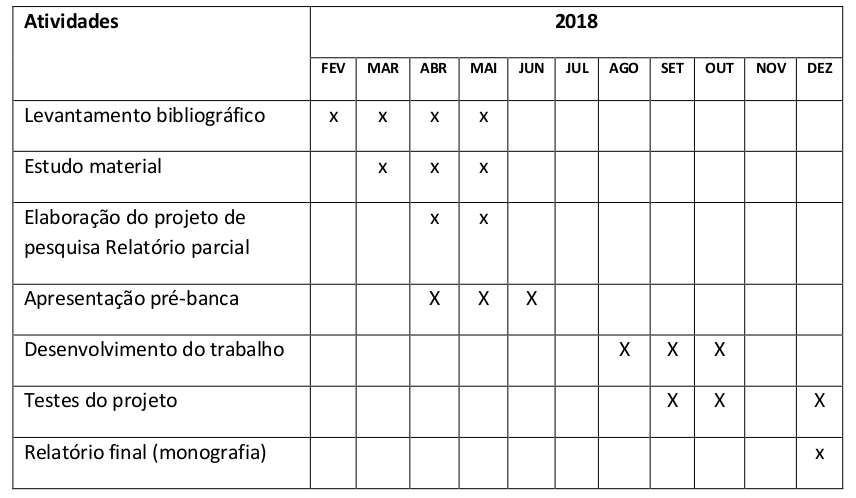
\includegraphics[width=1\textwidth]{cronograma.png}
\end{figure}

\newpage


% Uncomment the following two lines if you want to have a bibliography. Please do not forget to add an entry to your bibliography and reference it by using the \cite{} command
%\bibliographystyle{alphadin}
\providecommand*{\refname}{}
\renewcommand*{\refname}{\begin{center}\textbf{REFERÊNCIAS}\end{center}}

\newpage
%\vspace*{4cm}
%\providecommand{\bibname}{}
%\renewcommand{\bibname}{\begin{center}\textbf{REFERÊNCIAS}\vspace{48pt}\end{center}}

\pagestyle{empty}
\pagestyle{myheadings}

%\bibliographystyle{alpha}

\addcontentsline{toc}{section}{REFER\^ENCIAS}
\bibliography{bibliografia}
\nocite{Alves}
\nocite{Wordnet}
\nocite{Sentist}
\nocite{Sentw}
\nocite{Sailail}
\nocite{Vader}
\nocite{Sean}
\nocite{Rodrigo}
\nocite{liwc}
\nocite{Infografico}
\nocite{Gauchazh}
\nocite{Symeon}
\nocite{Research}

% End of the document
\end{document}
